%!TEX program = xelatex
%!BIB program = bibtex

\documentclass[en,black,12pt,normal]{elegantnote}
\usepackage{float}
\usepackage{subfigure}


\newcommand{\upcite}[1]{\textsuperscript{\textsuperscript{\cite{#1}}}}

\title{Practical 8 OMICS}
\author{WenYuan Jiang\\ID: 1951510}
\institute{School of Life Science, Tongji University}
%\version{1.00}
\date{\today}
\lstset{basicstyle=\footnotesize\ttfamily}
\AtBeginEnvironment{lstlisting}{\linespread{0.75}\selectfont}

\begin{document}

\maketitle

\section{Inrtoduction}

Researchers try to identify biomarkers for early detection and effective therapy of COVID-19 patients. 
Please search a transcriptome experiment taken from COVID-19 patients as well as healthy controls. 
To interpret how the host immune system responds to the infection of sars-cov2, please perform a transcriptomics analysis.

\subsection*{Hint:}

\begin{enumerate}
    \item Identify the DEGs (differentially expressed genes) among different groups (mild patient, 
    severe patient and healthy controls), list your filtering criteria and the number of DEGs. 
    Here, we only count coding transcripts.
    \item Draw Venn diagrams of upregulated or downregulated DEGs in mild, severe and healthy groups.
\end{enumerate}



\section{Please search a transcriptome experiment\dots}

The search and download process is done on \date{\today}.

According to the requirements, we searched in the \lstinline{GEO DataSets}, with the query \lstinline{COVID-19 patients}.

The query gives us \lstinline{2405} results, eg. \lstinline{Genome-wide DNA methylation analysis of COVID-19 severity}. 
For the convenience of further analysis, 
we narrow down the datasets to those produced by microarray (\lstinline{Expression profiling by array}).

This filter gives us two results, and we choose the \textbf{The transcriptional profiles of severe COVID-19}
as our dataset (\lstinline{Gene Expression Omnibus (GEO) and GSE164805}).\upcite{barrett2012ncbi}

The experiment is published in Front. Immunol., on 18 February 2021, 
titled \textit{Inflammation and Antiviral Immune Response Associated With Severe Progression of COVID-19}.\upcite{fimmu2021}

\section{Identify the DEGs\dots}

To avoid writing code in R, which is a program language for data analysis, the authors used the web service \lstinline{GEO2R},
to analysis the dataset.

Type the accession number \lstinline{GSE164805} in to the \lstinline{GEO2R} website
and then group the dataset as we needed. The figure of the gruops is shown below.

\begin{figure}[H]
    \centering
    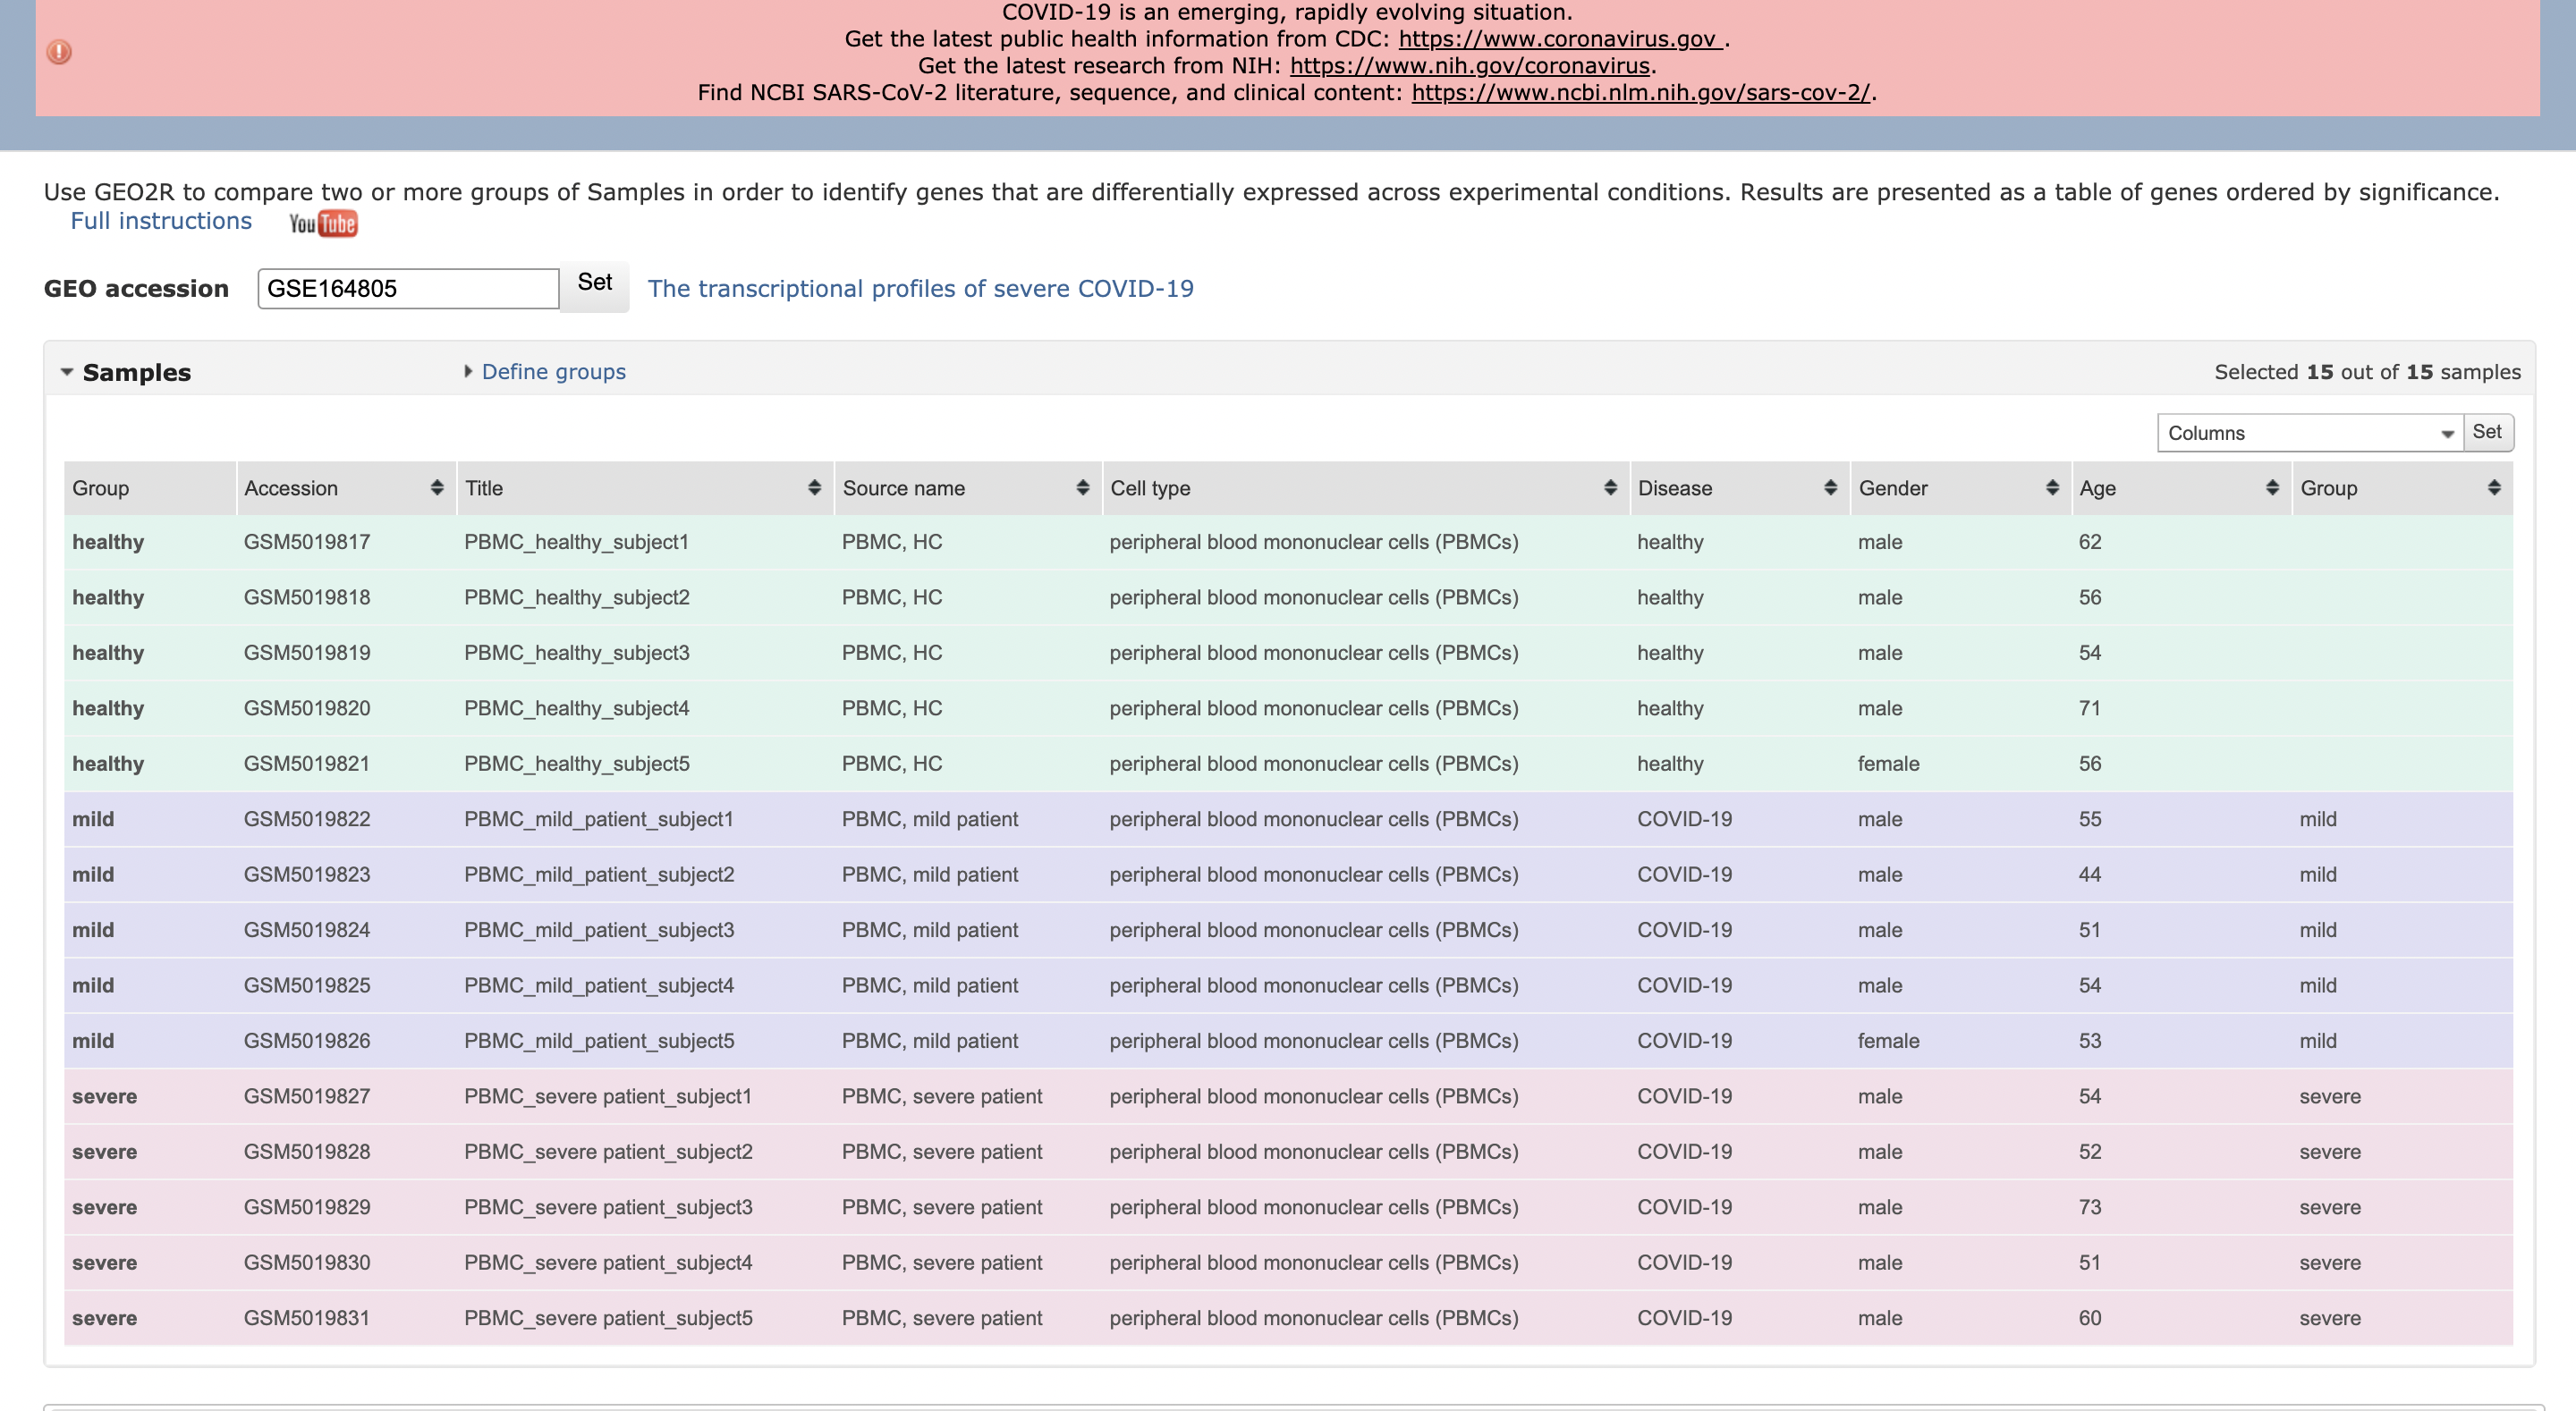
\includegraphics[width=1\textwidth]{G1}
    \caption{Groups of the analysis}
    \label{G1}
\end{figure}

Then run the analysis with the default parameters. The overview of the results are shown in the figure below.

\begin{figure}[H]
    \centering
    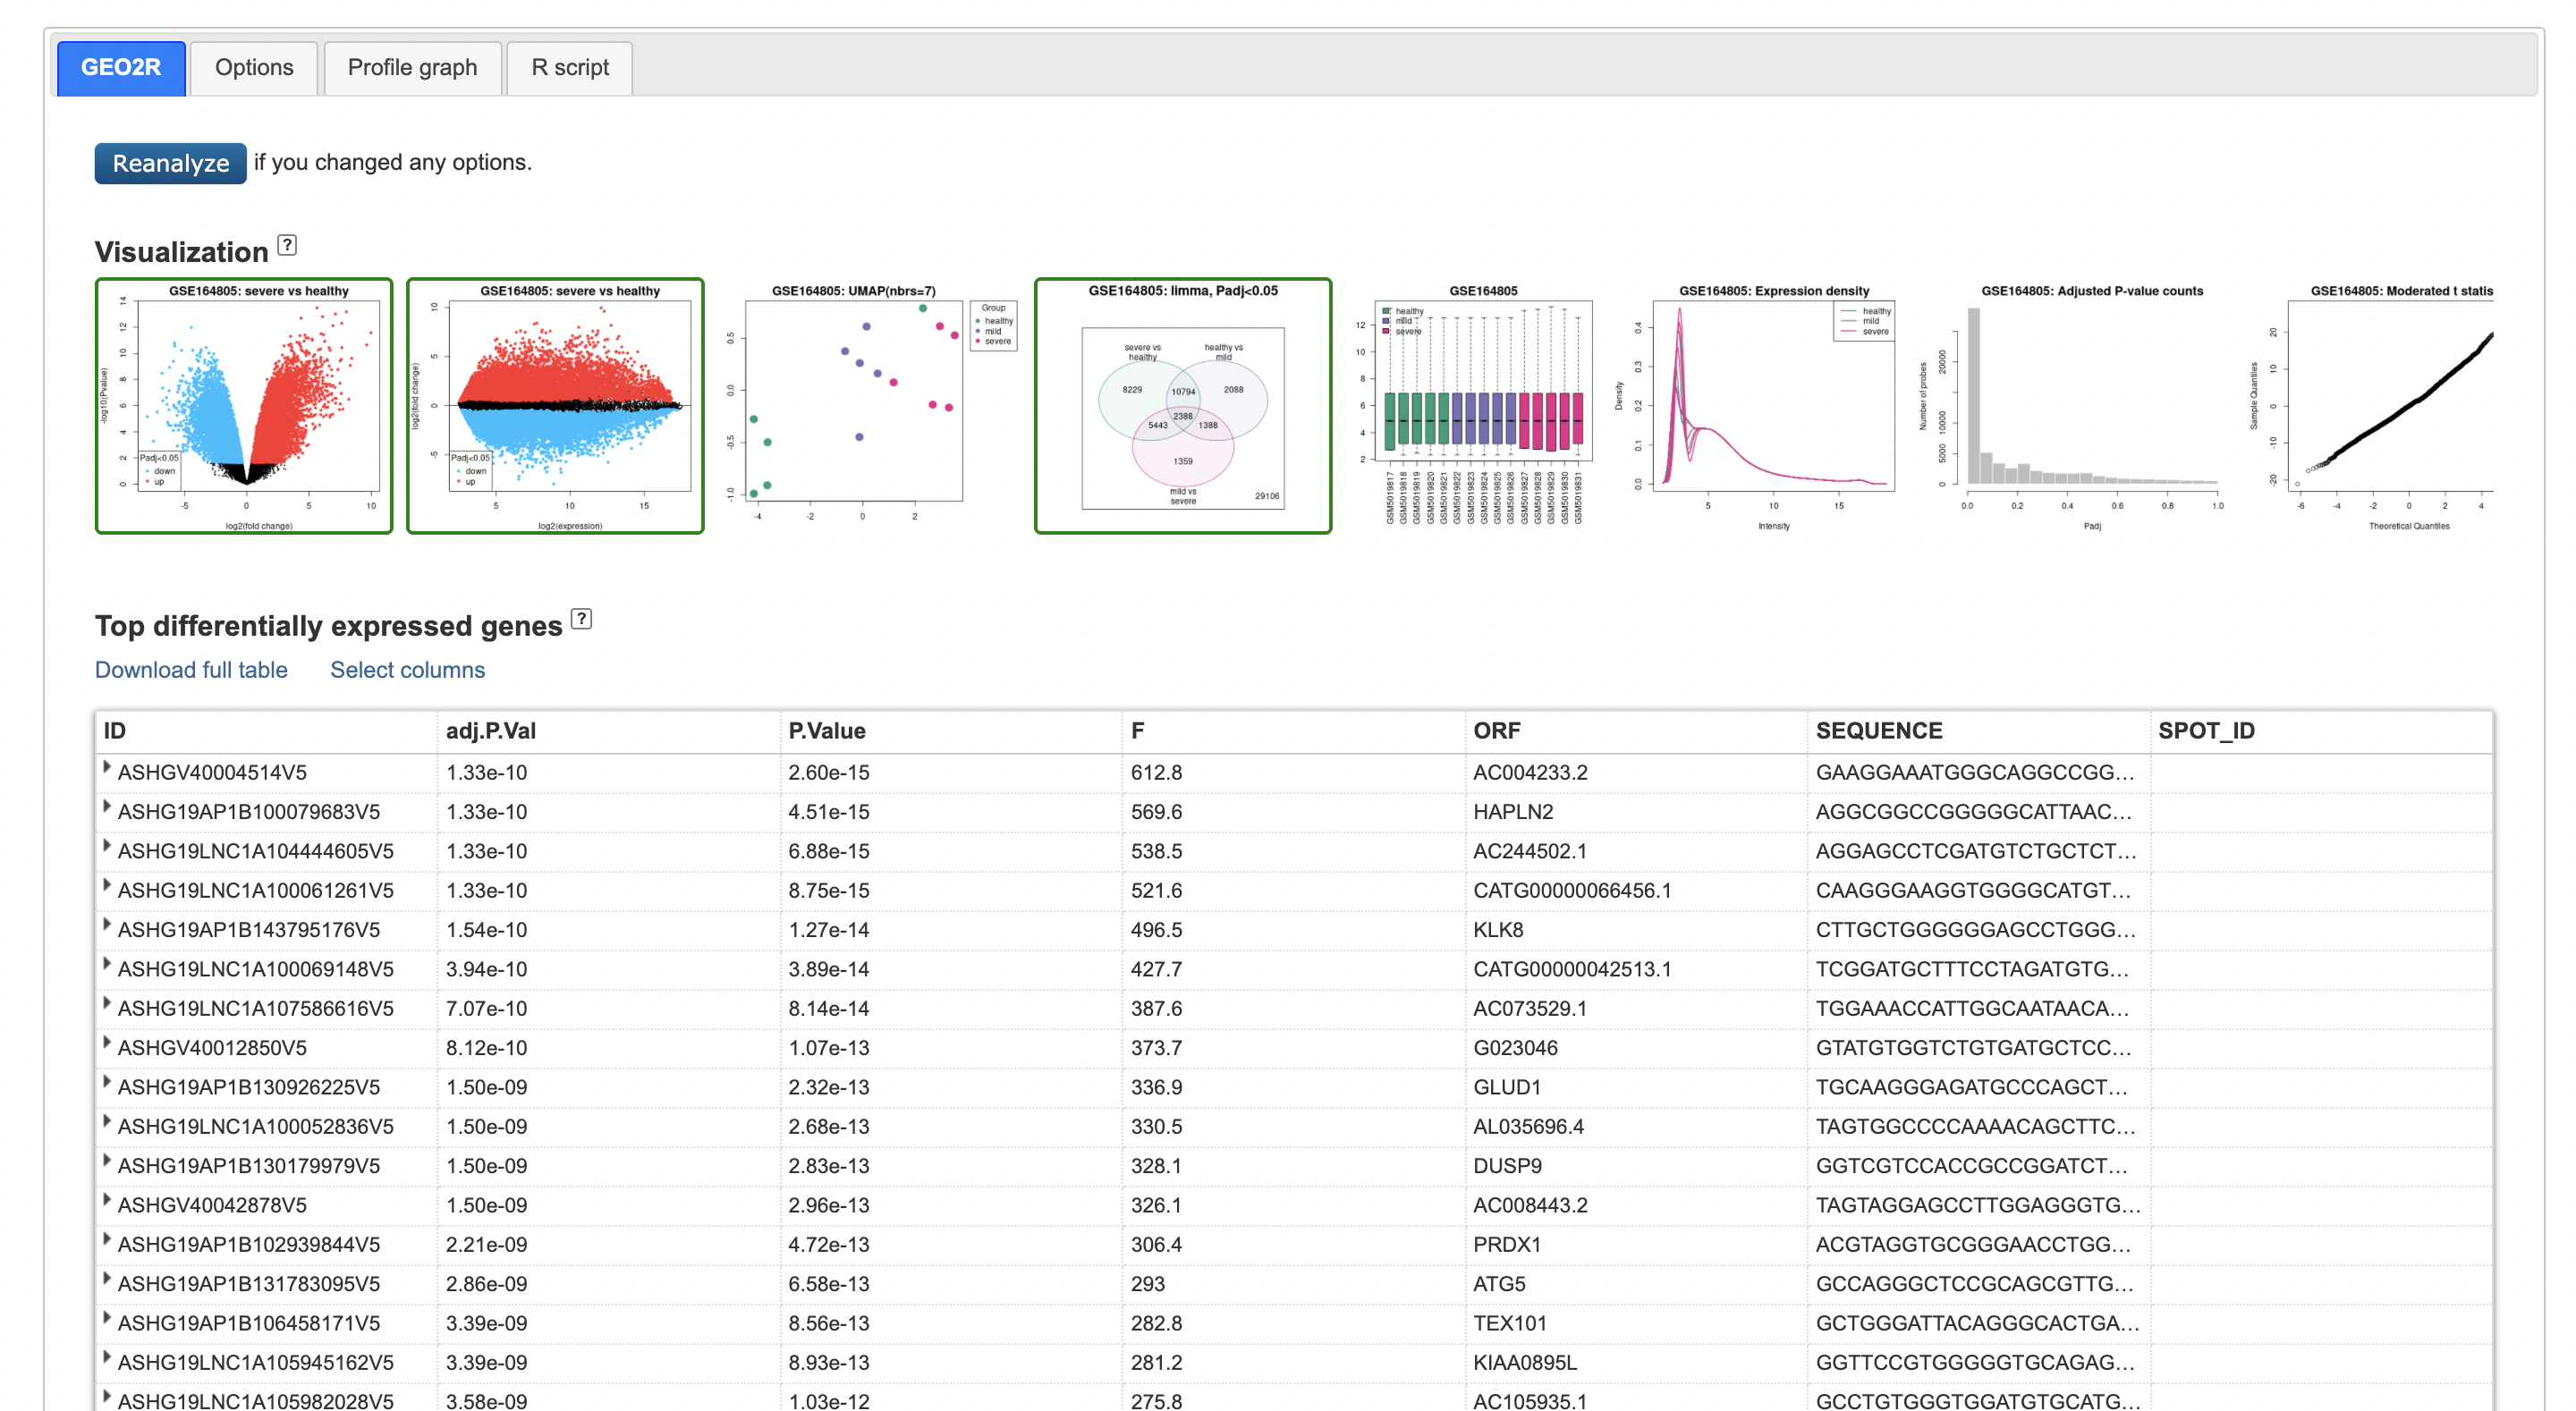
\includegraphics[width=1\textwidth]{G2}
    \caption{Results overview}
    \label{G2}
\end{figure}

In default parameters, Significance level cut-off is set to \lstinline{0.05}.
More detailed parameters is shown below.

\begin{itemize}
    \item Apply adjustment to the P-values: Benjamini \& Hochberg (False discovery rate)
    \item Apply log transformation to the data: Auto-detect
    \item Apply limma precision weights (vooma): No
    \item Force normalization: No
    \item Significance level cut-off: 0.05
\end{itemize}

We set the Significance level cut-off to \lstinline{0.001}, and run the analysis again.
Raw data of the top 250 results is listed in the Supplementary.

Among the top 250 results, 89 of them are well annotated, protein coding gene, and the examples are listed below.

\begin{lstlisting}
                     =====ORF NAME=====
"CATG00000015125.1" "CATG00000023238.1" "CATG00000028059.1" 
"CATG00000062999.1" "RALGAPA2"          "TULP2"            
"KCNJ2"             "MAGEA10"           "ARHGEF9"           
"HAPLN2"            "USP44"             "PRDX1"            
"SEPT12"            "RPL3L"             "LCN9"              
"RPS3"              "TMEM143"           "UBXN1"            
"CPA3"              "IRF2BP1"           "CHST1"             
"TMOD3"             "KRT2"              "TIGD3"            
"MOS"               "C3orf80"           "TMEM151A"          
"MARCKSL1"          "CREB3L2"           "PGP"              
"PSMF1"             "ARHGEF1"           "CERKL"             
"SAXO2"             "DUSP9"             "RBM5"             
"DUS1L"             "MAK"               "TBCD"              
"LRRC61"            "FAM189B"           "SIPA1L2"          
"RASAL2"            "S100A16"           "ATG5"              
"CNNM2"             "MUTYH"             "EXOSC2"           
"TNNC2"             "IFT52"             "F10"               
"TMEM252"           "HES5"              "EDN1"             
"STRN4"             "NDUFA4L2"          "UMOD"              
"TMEM106B"          "EMC6"              "LONRF1"           
"PXMP4"             "LLCFC1"            "AP2M1"             
"EIF4G1"            "TLR6"              "PPP1R12A"         
"BTBD19"            "ILDR1"             "ZNF706"            
"BEAN1"             "ZFP37"             "GJD3"             
"PPY"               "TEX101"            "SALL2"             
"GCSAML-AS1"        "SMTN"              "TMEM114"          
"FGF1"              "CATG00000116804.1" "CATG00000057159.1" 
"CATG00000039615.1" "CATG00000054736.1" "CATG00000058631.1"
"KIF27"             "KLK8"              "SP140"             
"TRIM6"             "GLUD1"            
\end{lstlisting}

Moreover, there are 20727 coding genes in the dataset, and in the following analysis,
we will analysis all the 20727 genes instead of those top significant ones.

\section{Draw Venn diagrams\dots}
In the venn diagrams, we will show the results from all the 20727 genes.


\subsection{Differentially expressed genes}
Venn diagrams of the differentially expressed genes of all coding genes is shown below.
\begin{figure}[H]
    \centering
    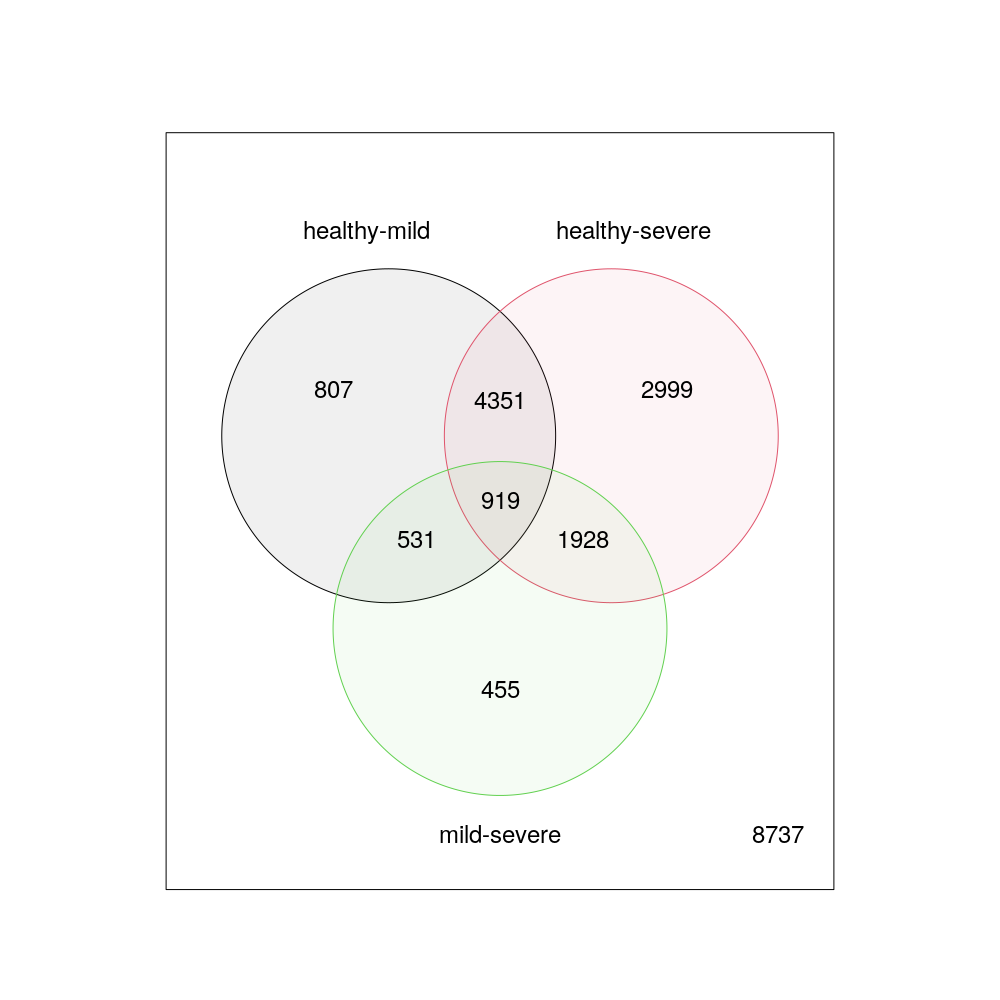
\includegraphics[width=0.7\textwidth]{AllCodingVenn1}
    \caption{Differentially expressed genes}
    \label{VA}
\end{figure}


Among these 20727 genes, 919 genes are differently expressed in different groups.
Among these genes, 66 of them are in the top 250 list, indicating that
they are related to the interpretation of how the host immune system responds to the infection of sars-cov2.

\subsection{Upregulated DEGs}
Venn diagrams of the upregulated DEGs of all coding genes is shown below.

\begin{figure}[H]
    \centering
    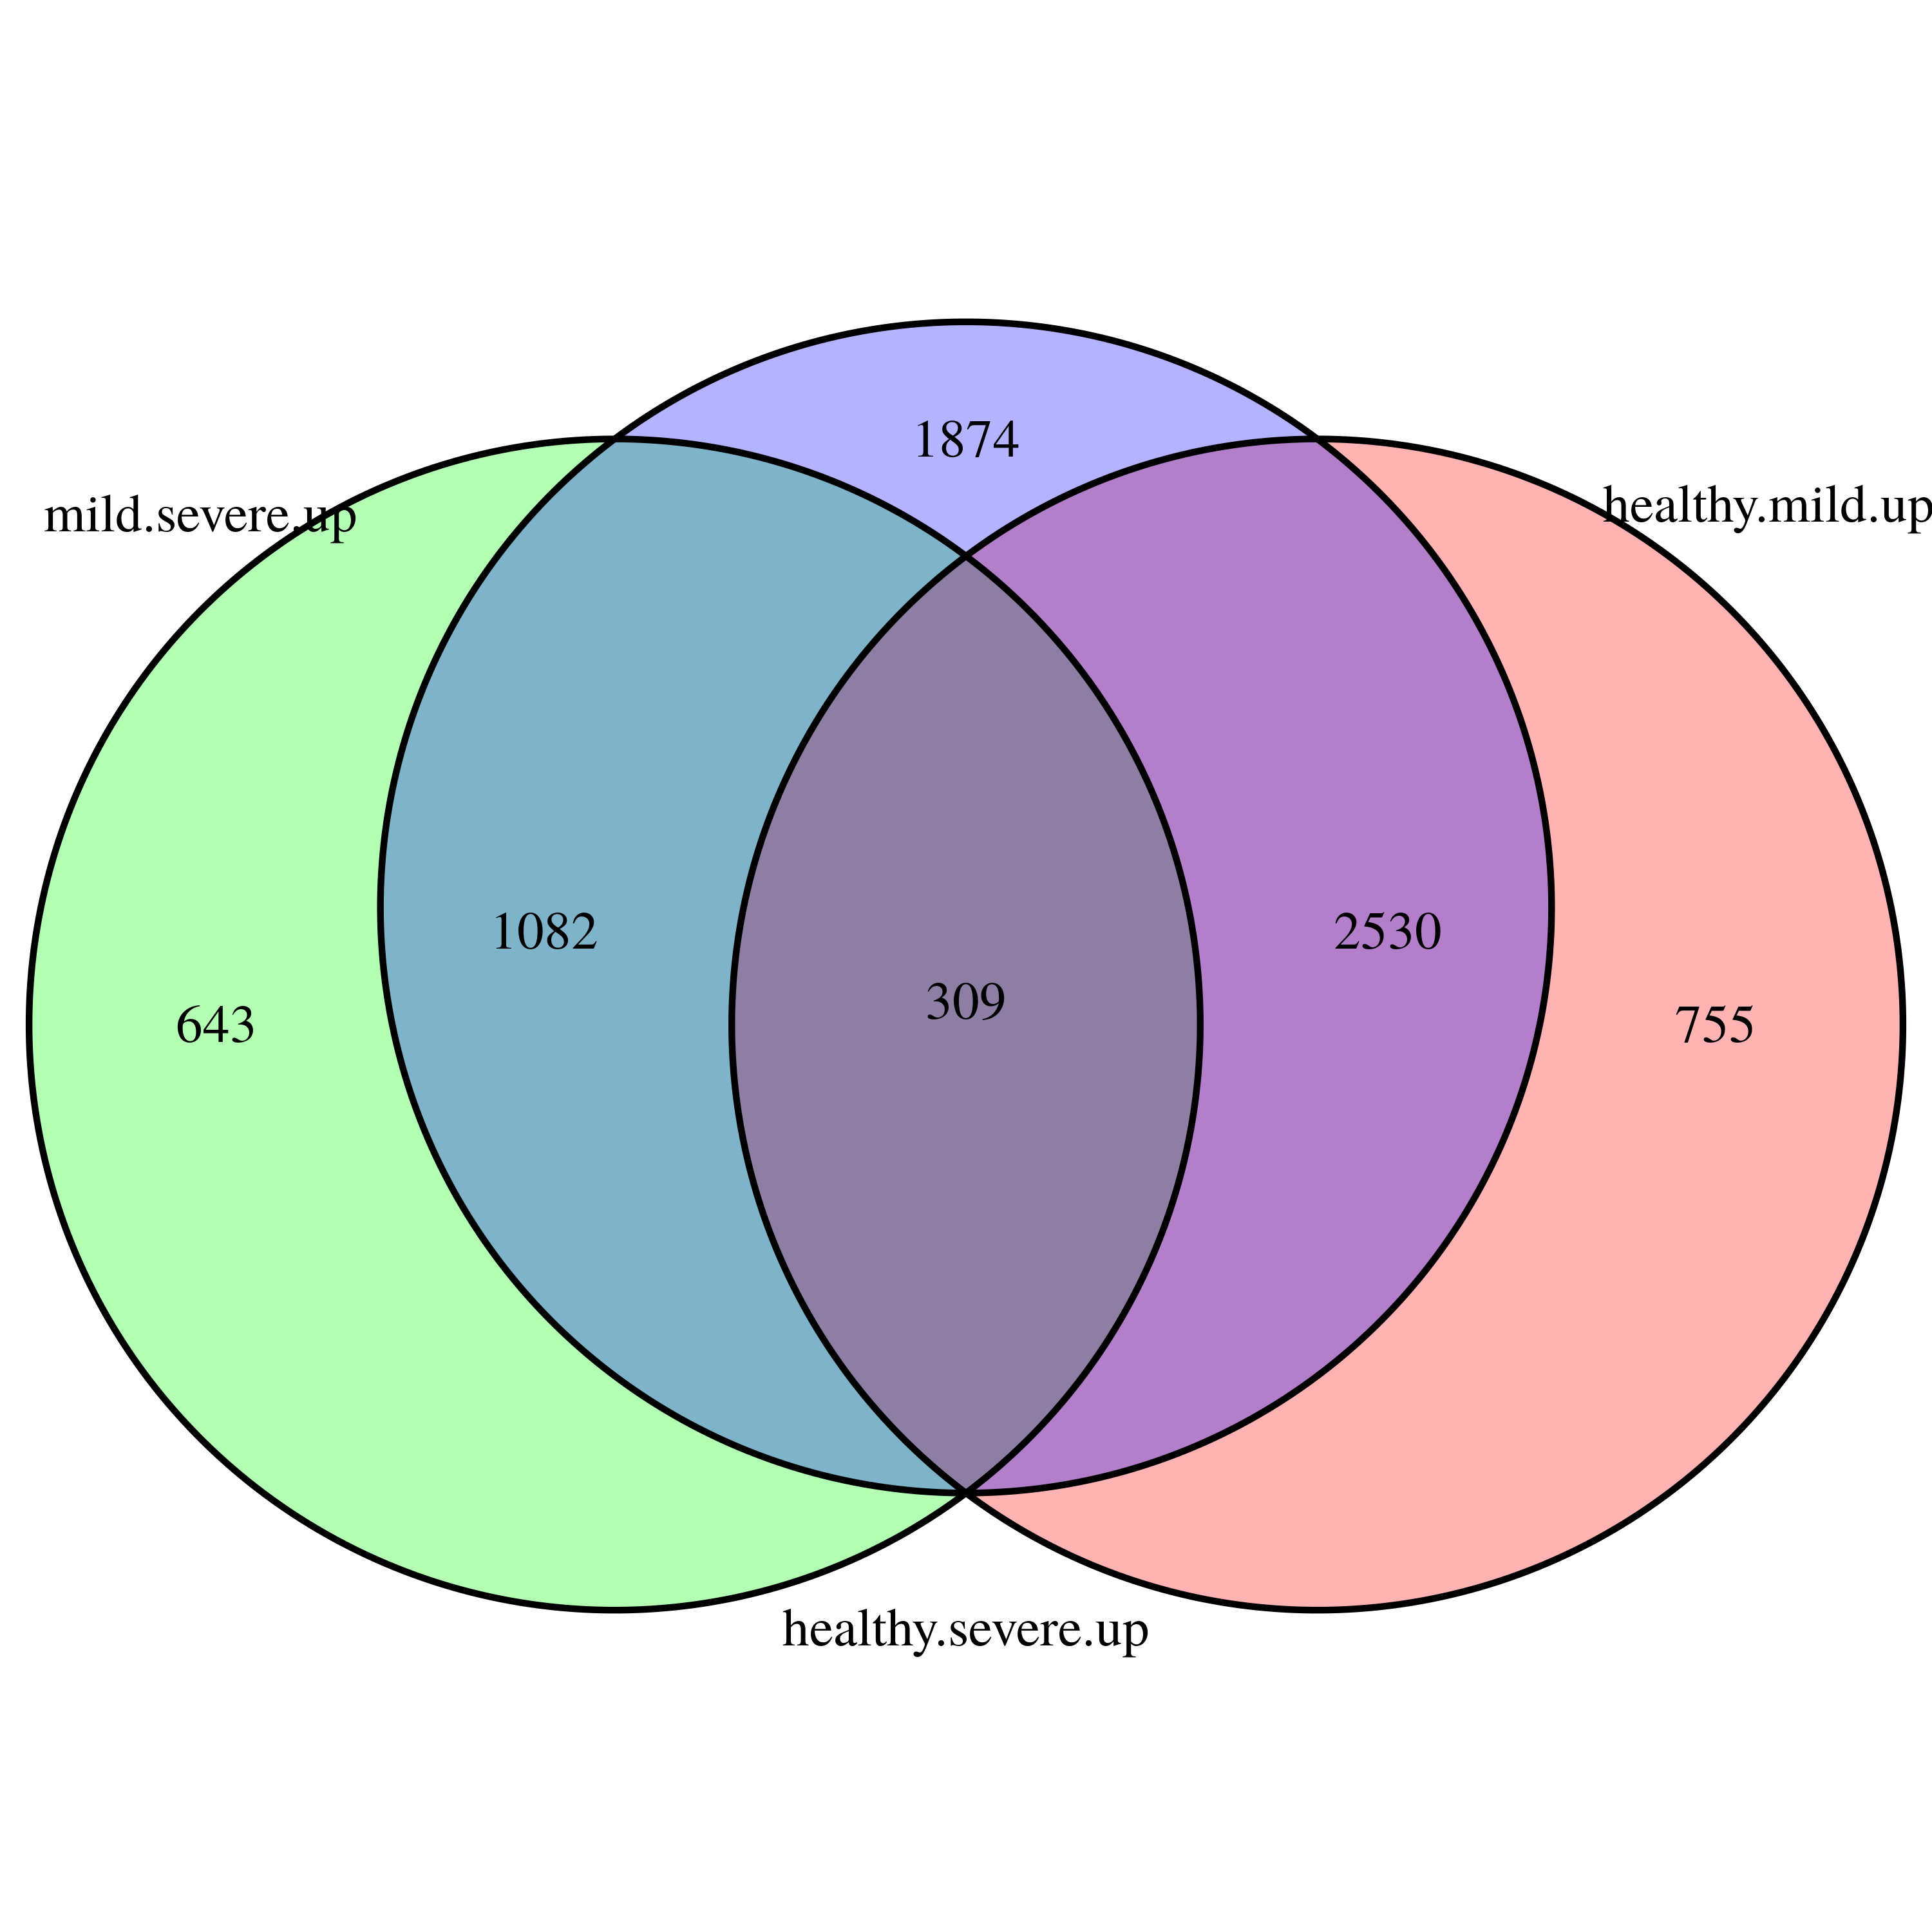
\includegraphics[width=0.7\textwidth]{venn_up_code}
    \caption{Upregulated DEGs}
    \label{VU}
\end{figure}


\subsection{Downregulated DEGs}
Venn diagrams of the downregulated DEGs of all coding genes is shown below.

\begin{figure}[H]
    \centering
    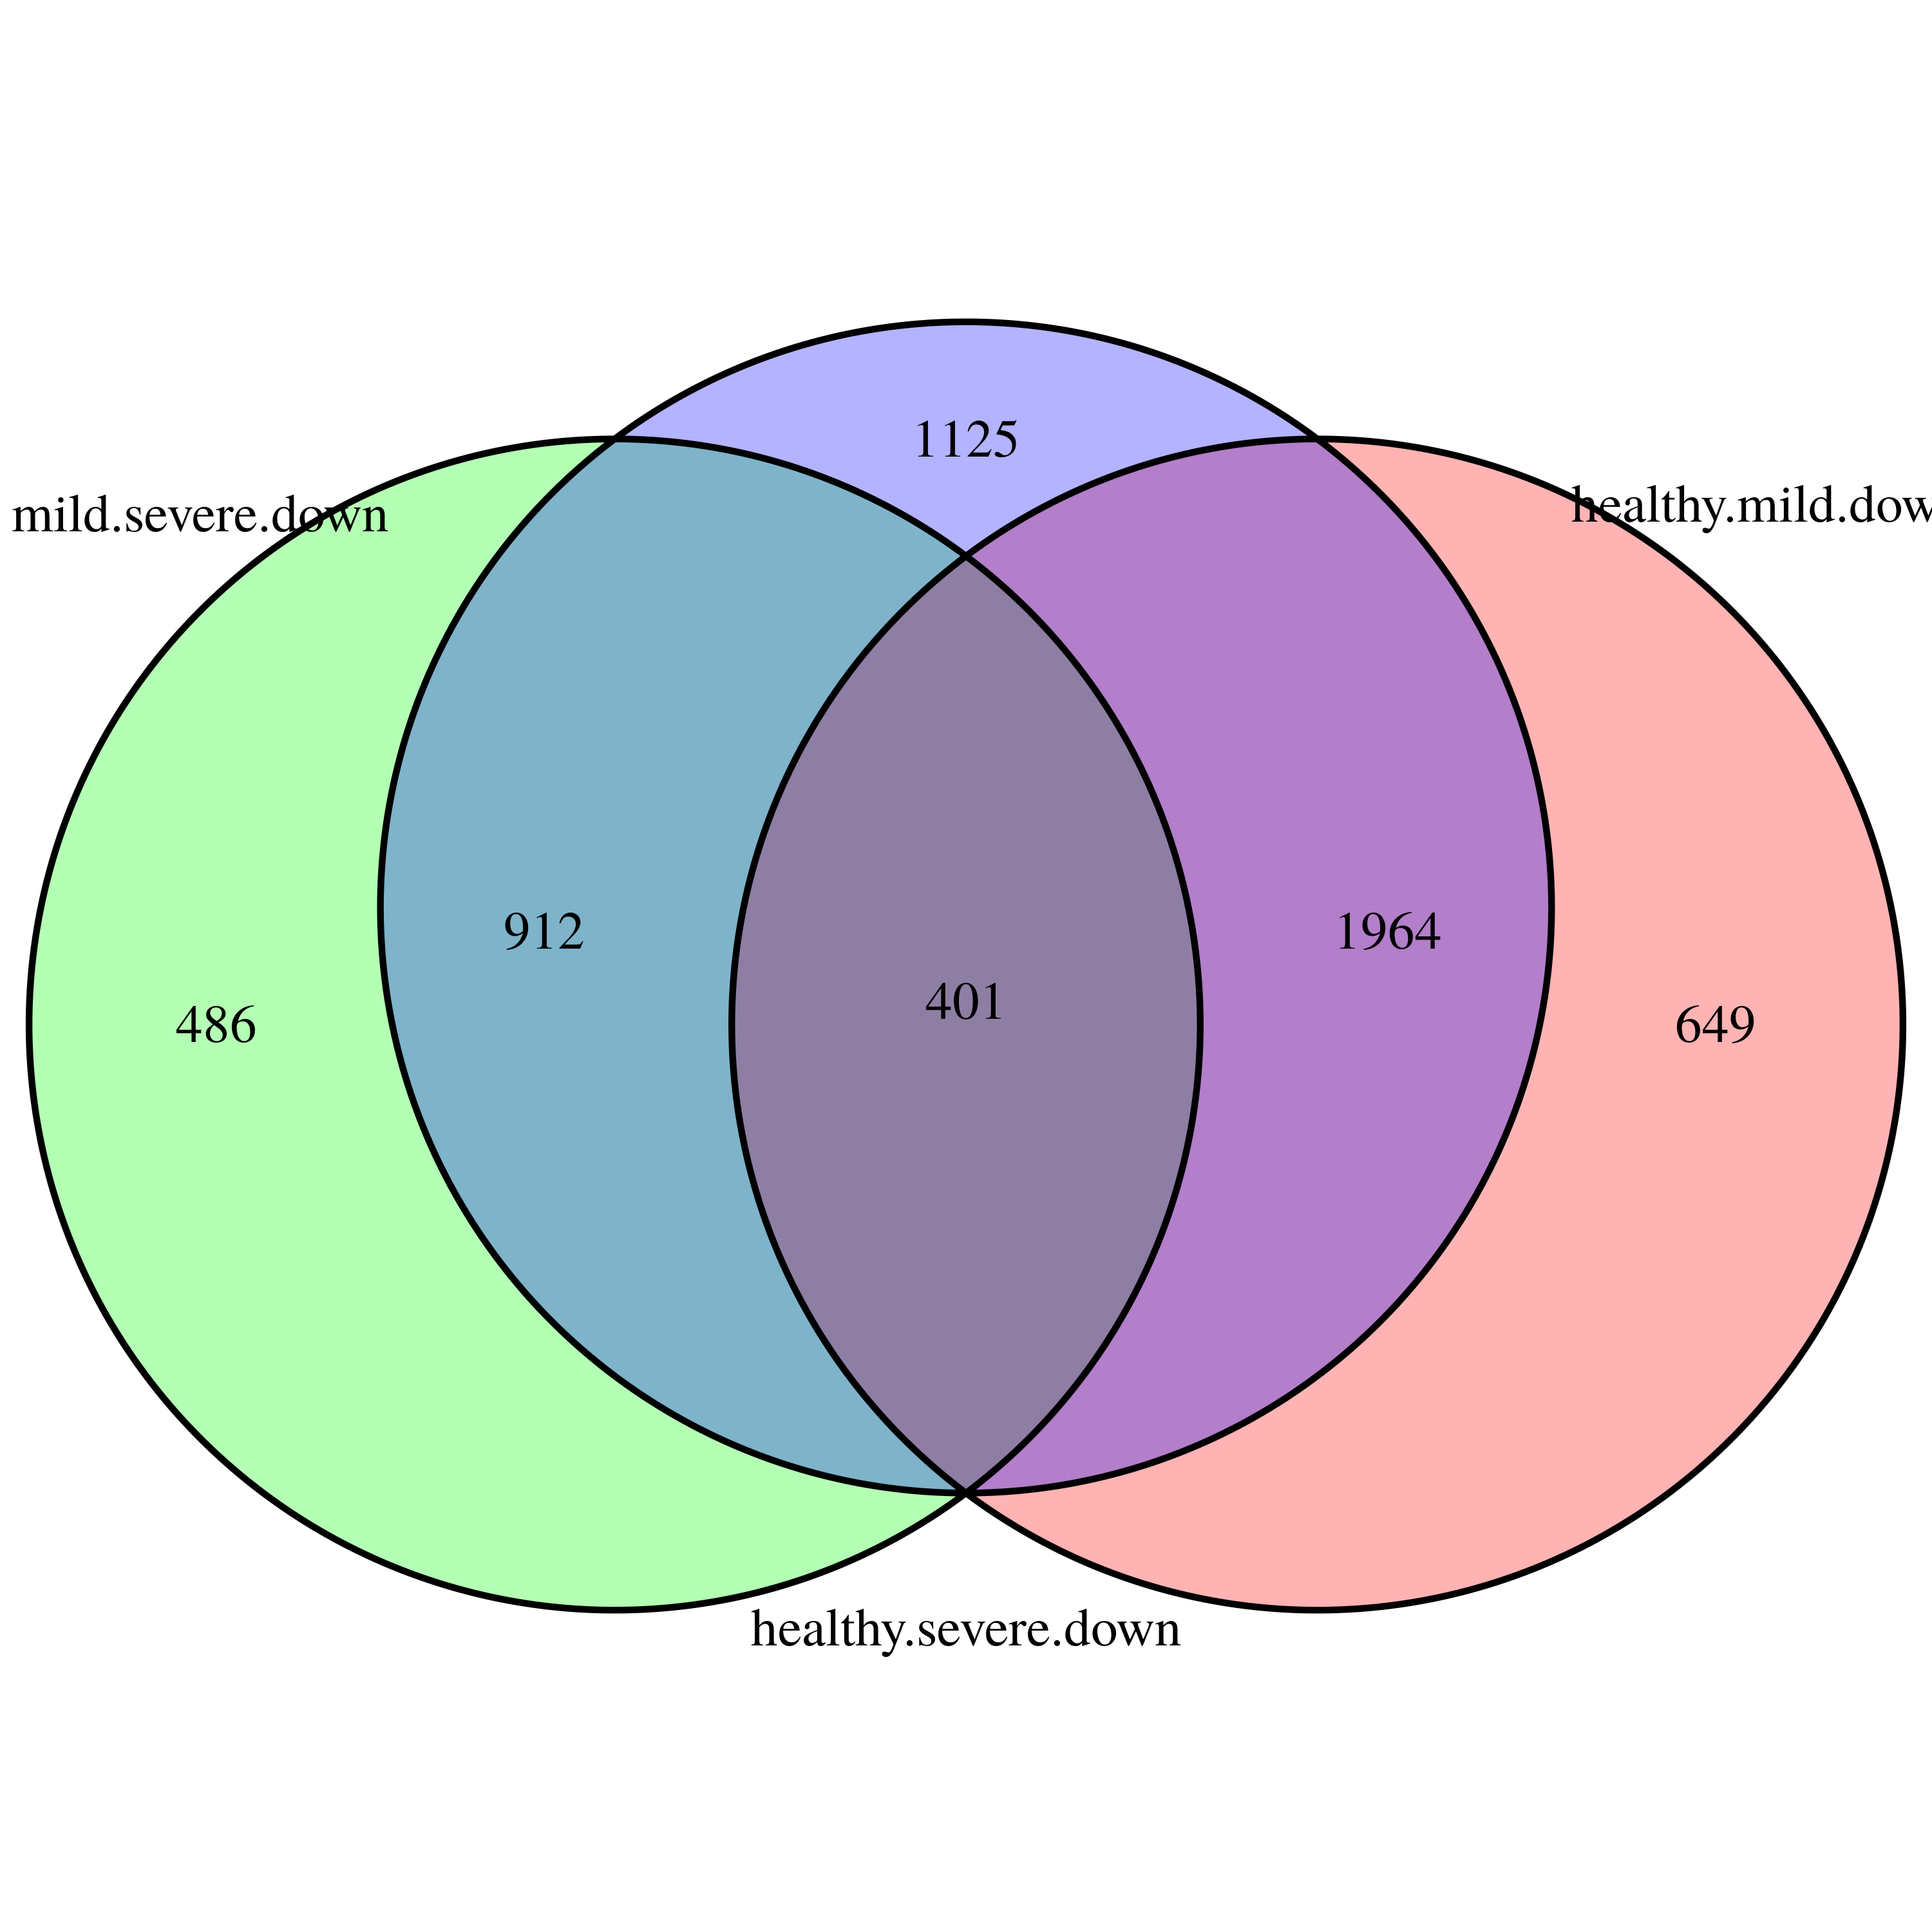
\includegraphics[width=0.7\textwidth]{venn_down_code}
    \caption{Downregulated DEGs}
    \label{VD}
\end{figure}

\subsection{Comments}

\section{Other results}
Compared with the results in the previous paper,
the overall ratio of different part of the venn graph
is similar, in spite of the fact that we did not limit our
analysis to the most significant results.


\subsection{Quality control of the analysis}

The P-value counts figure is shown below.
The shape of the graph shows that the results are desirable.

\begin{figure}[H]
    \centering
    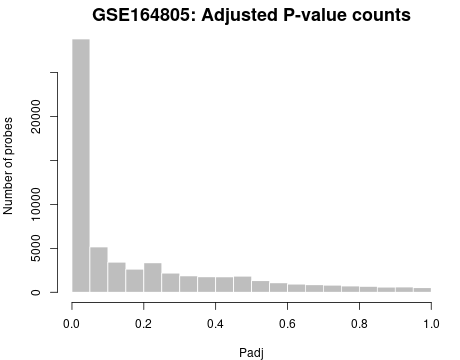
\includegraphics[width=0.7\textwidth]{Pv}
    \caption{The P-value counts}
    \label{PV}
\end{figure}

\subsection{All coding genes}
The heatmap of all coding genes is shown below.

\begin{figure}[H]
    \centering
    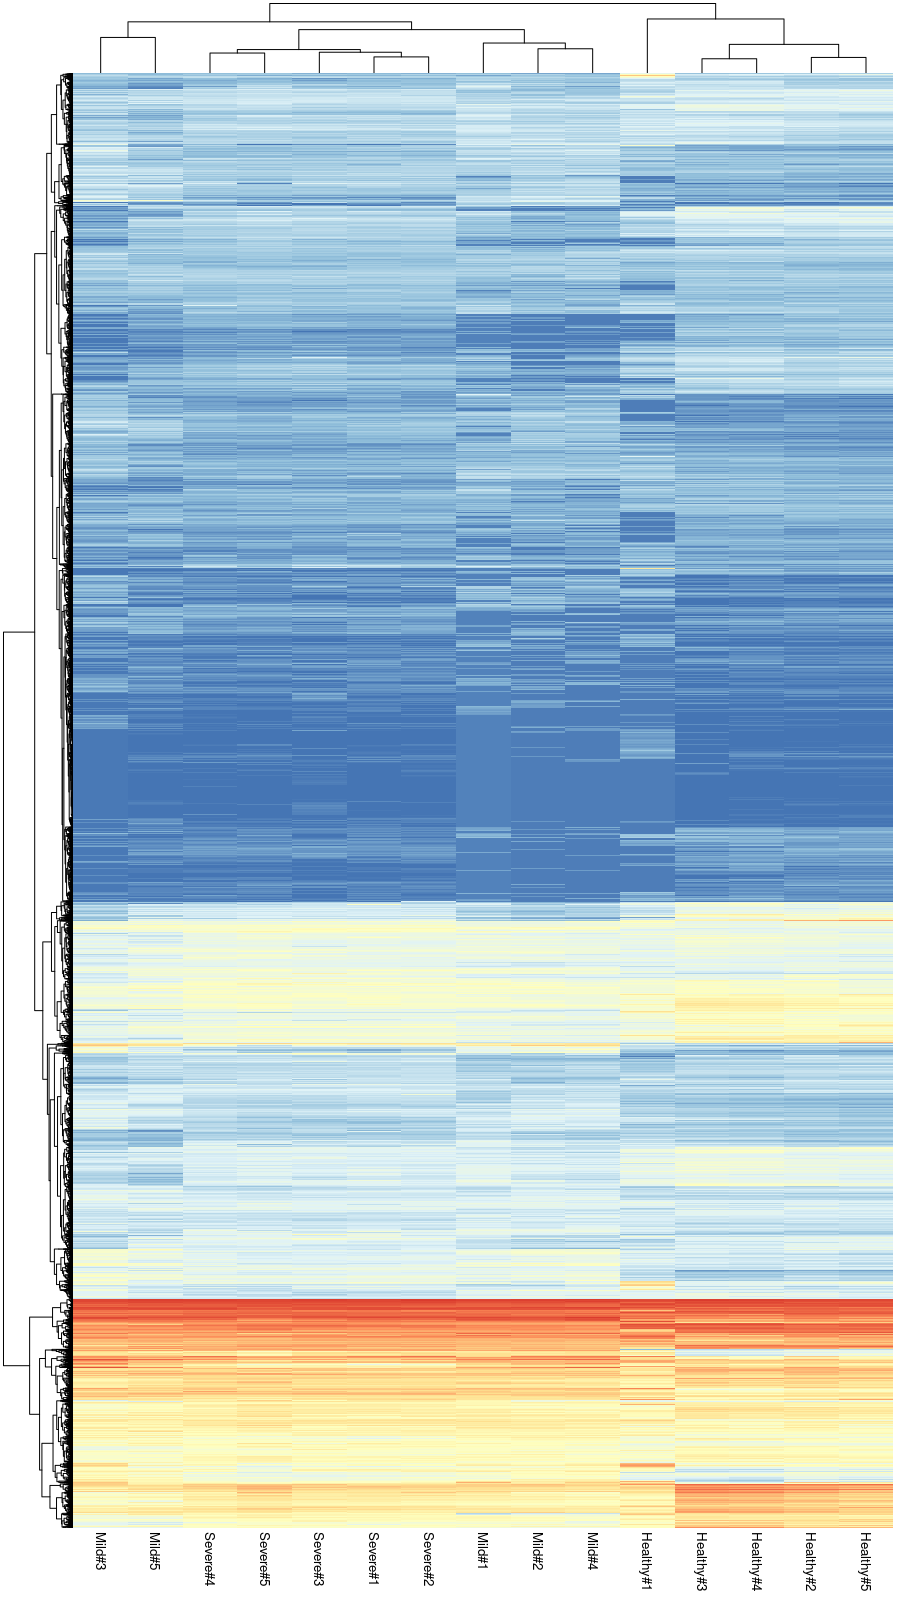
\includegraphics[width=0.5\textwidth]{AllCodingGenes}
    \caption{Heatmap of all coding genes}
    \label{ACG}
\end{figure}

No significant difference can be seen, 
and the results by the clustering algorithm is not reasonable.


\subsection{Top 89 coding genes}
The heatmap of top 89 coding genes is shown below.

\begin{figure}[H]
    \centering
    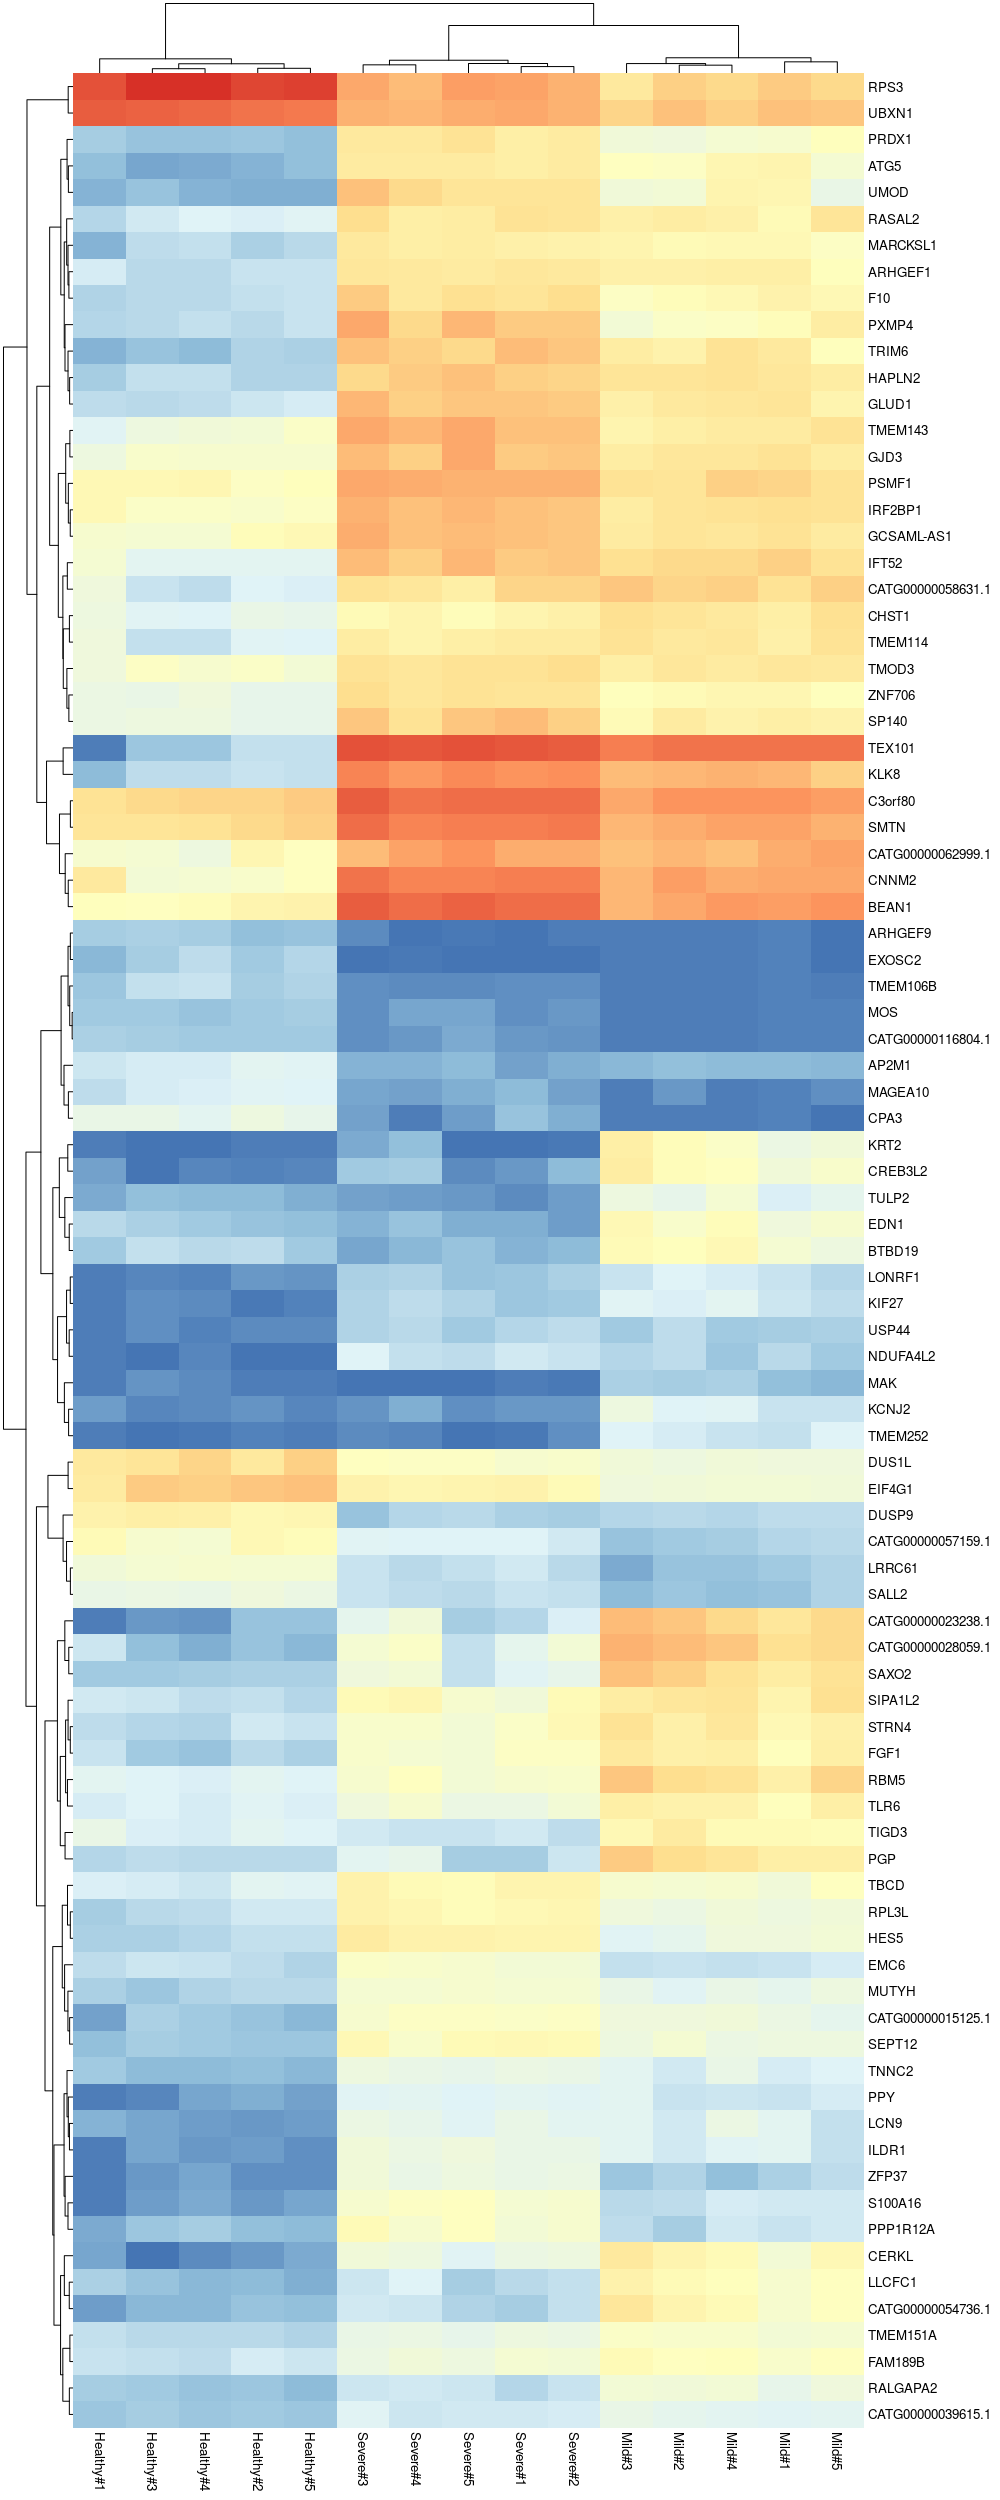
\includegraphics[width=0.5\textwidth]{TopCodingGenes}
    \caption{Heatmap of top 89 coding genes}
    \label{TCG}
\end{figure}

This time significant difference can be seen, 
and the the clustering algorithm gives reasonable results.





























































\bibstyle{unsrt}
\bibliography{references}{}
\end{document}
